\documentclass{stdlocal}
\begin{document}
\section{Mathematical Preliminaries} % (fold)
\label{sec:preliminaries}

To systematically approach the topic of curve smoothing algorithms for surface meshes, basic knowledge in the topics of differential geometry for curves and its further application and generalization to polyhedral surfaces is administrable.
% It allows to rigorously generalize the concept of geodesics to discete surfaces and formulate their initial and boundary value problems.
% Geodesics can be interpreted as the class of smoothest curves and as such they build the foundation of curve smoothing algorithms.
As modern differential geometry heavily builds on the mathematical tools given in the area of analysis on manifolds, the reader is assumed to be familiar with its basic concepts.
For convenience, section~\ref{sec:analysis_on_manifolds} in the appendix provides a brief introduction to clarify and remind of notations.
% In the following, a brief overview of the main concepts is given.

\subsection{Differential Geometry of Curves} % (fold)
\label{sub:differential_geometry}

  The theory of smooth curves in space or smooth surfaces is one of the main concerns of classical differential geometry.
  Therefore, we refer to some standard textbooks, namely \textcite{goldhorn2009}, \textcite{carmo2016}, \textcite{kuehnel2013}, and \textcite{stahl2013}, for a more excessive and thorough introduction on this topic.
  For the purpose of consistent notation and as a reminder, the main concepts of smooth curves are briefly given in the following in the sense of classical and modern differential geometry based on these books.

  In the fields of analysis and numerical mathematics, it is a natural approach to extend a well-founded and -understood theory for smooth objects to their discrete counterparts and vice versa.
  Hereby, discrete or smooth objects will be typically characterized by the limit of sequences of smooth or discrete objects, respectively.
  This procedure may then allow for a generalization of properties and statements from one to the other case.
  Surface mesh curves, as they will be defined in section~\ref{sub:polyhedral_surfaces}, can exactly be seen as such discrete counterparts to the shapes of special classes of smooth parameterized curves \autocite{polthier2006}. \\
  \autocite{forster2016,elstrodt2011,cheney2008,goldhorn2009}

  \begin{definition}[Open and Closed Parameterized Curves]
    Let $n\in\setNatural$, $k\in\setNatural_{\infty}$, and $[a,b]\subset\setReal$ be a compact interval.\\

    An (open) ($n$-dimensional) (parameterized) curve (of class $\mathrm{C}^k$) is a $k$-times continuously differentiable function $\function{γ}{[a,b]}{\setReal^n}$ on the compact interval $[a,b]$. \\

    A closed ($n$-dimensional) (parameterized) curve (of class $\mathrm{C}^k$) is a $k$-times continuously differentiable function $\function{γ}{\mathds{T}^1[a,b]}{\setReal^n}$ on the respective one-dimensional topological torus $\mathds{T}^1[a,b]$. \\

    Parameterized curves of class $\mathrm{C}^\infty$ are also called smooth.
  \end{definition}
  In the sense of this definition, a curve needs to at least provide some kind of smoothness in the form of continuous differentiability.
  Trying only to rely on a continuity property, the definition would also include pathological cases, such as space-filling curves that cover a whole square in the plane \autocite{kuehnel2013}.
  Other generalizations therefore rely on the use of either rectifiable or piecewise continuously differentiable curves.

  Defining closed curves to be smooth functions on the topological space of a one-dimensional torus is a technicality that automatically takes care of the agreement of values and derivatives at the two boundary points which are glued together \autocite{stahl2013,carmo2016}.
  The change of topological requirements for a closed curve still allows to interpret it as a general curve.
  For this reason, when referring to parameterized curves, both closed and open curves are meant.
  To get an impression of the implications of this definition, in figure~\ref{fig:curve-examples} typical examples of smooth curves are shown.

  \begin{figure}[t]
    \centering
    \begin{subfigure}[t]{0.32\linewidth}
      \center
      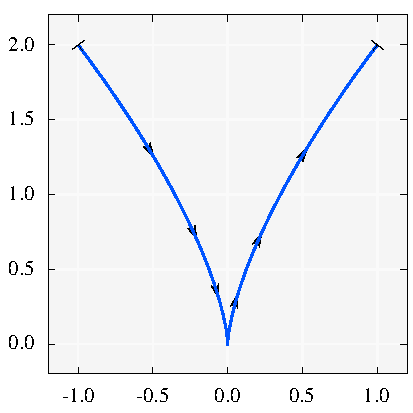
\includegraphics[width=\linewidth]{plots/curve-example-1.pdf}
      \caption{%
        Semicubical Parabola
        \[
          \begin{aligned}[t]
            &\function{γ}{[-1,1]}{\setReal^2} \\
            &γ(t) \define
            \begin{pmatrix}
              t^3 \\
              2t^2
            \end{pmatrix}
          \end{aligned}
        \]
      }
    \end{subfigure}
    \begin{subfigure}[t]{0.32\linewidth}
      \center
      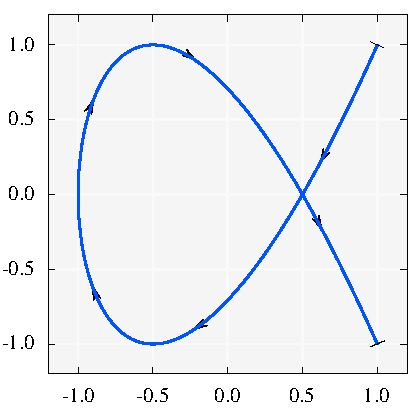
\includegraphics[width=\linewidth]{plots/curve-example-3.pdf}
      \caption{%
        Lissajous Curve
        \[
          \begin{aligned}[t]
            &\function{γ}{[0,2π]}{\setReal^2} \\
            &γ(t) \define
            \begin{pmatrix}
              \cos t \\
              \cos\roundBrackets{\frac{3}{2}t}
            \end{pmatrix}
          \end{aligned}
        \]
      }
    \end{subfigure}
    \begin{subfigure}[t]{0.32\linewidth}
      \center
      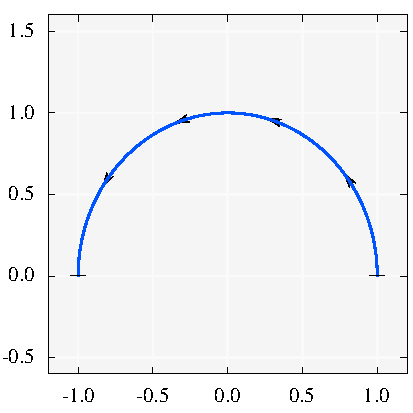
\includegraphics[width=\linewidth]{plots/curve-example-5.pdf}
      \caption{%
        Half-Circle
        \[
          \begin{aligned}[t]
            &\function{γ}{[0,π]}{\setReal^2} \\
            &γ(t) \define
            \begin{pmatrix}
              \cos t \\
              \sin t
            \end{pmatrix}
          \end{aligned}
        \]
      }
    \end{subfigure}

    \begin{subfigure}[t]{0.32\linewidth}
      \center
      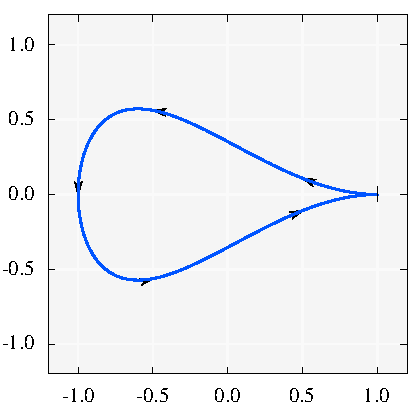
\includegraphics[width=\linewidth]{plots/curve-example-2.pdf}
      \caption{%
        Teardrop Curve
        \[
          \begin{aligned}[t]
            &\function{γ}{\mathds{T}^1[0,2π]}{\setReal^2}\\
            &γ(t) \define
            \begin{pmatrix}
              \cos(t) \\
              \sin(t)\sin^3\roundBrackets{\frac{1}{2}t}
            \end{pmatrix}
          \end{aligned}
        \]
      }
    \end{subfigure}
    \begin{subfigure}[t]{0.32\linewidth}
      \center
      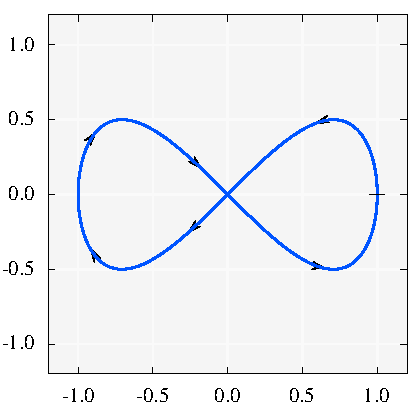
\includegraphics[width=\linewidth]{plots/curve-example-4.pdf}
      \caption{%
        Lissajous Curve
        \[
          \begin{aligned}[t]
            &\function{γ}{\mathds{T}^1[0,2π]}{\setReal^2} \\
            &γ(t)\define
            \begin{pmatrix}
              \cos t \\
              \frac{1}{2} \sin 2t
            \end{pmatrix}
          \end{aligned}
        \]
      }
    \end{subfigure}
    \begin{subfigure}[t]{0.32\linewidth}
      \center
      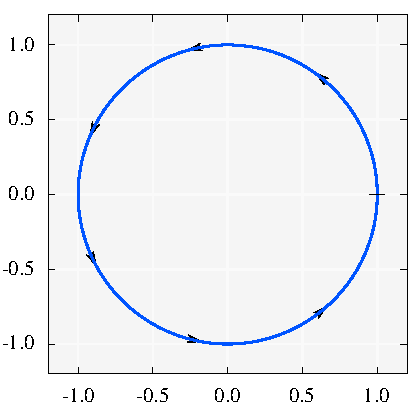
\includegraphics[width=\linewidth]{plots/curve-example-6.pdf}
      \caption{%
        Circle
        \[
          \begin{aligned}[t]
            &\function{γ}{\mathds{T}^1[0,2π]}{\setReal^2} \\
            &γ(t)\define
              \begin{pmatrix}
                \cos t \\
                \sin t
              \end{pmatrix}
          \end{aligned}
        \]
      }
    \end{subfigure}
    \caption[Examples of Smooth Parameterized Curves]{%
      \textbf{Examples of Smooth Parameterized Curves}\\
      All the plots show a smooth two-dimensional parameterized curve γ of a different class.
      The first row from left to right shows a general curve, a regular curve with self-intersection, and a regular and simple curve parameterized by arc length.
      The second row shows closed counterparts, respectively.
      Hereby, the black arrows indicate the orientation of the chosen parameterization and the black lines its start and end.
    }
    \label{fig:curve-examples}
  \end{figure}

  For most of the considered applications, the actual parameterization of a curve is not essential.
  Only the shape, given by its image, is used, referred to, and transformed.
  But using the shape and neglecting the parameterization of a curve does only make sense if the shape at least fulfills the properties of a one-dimensional manifold.
  Unfortunately, as can be seen in figure~\ref{fig:curve-examples}, the shape of parameterized curves may exhibit more general structures, such as sharp edges and self-intersections, and, thus, does not necessarily abide to these constraints.
  As a consequence, more regular and specialized classes of curves need to be looked at. \\
  \autocite{goldhorn2009,carmo2016,kuehnel2013}

  \begin{definition}[Regular and Simple Parameterized Curves]
    Let γ be a parameterized curve.
    Then γ is said to be simple if it is injective and regular if the following statement holds.
    \[
      \forall t\in \mathscr{D}(γ)^\circ \colon\quad γ'(t)\neq 0
    \]
    Furthermore, if $\norm{γ'} = 1$ then γ is parameterized by arc length.
  \end{definition}
  The definition states that the derivative of a regular curve is, apart from its boundary, never zero and therefore a map of full-rank at every inner point.
  Hence, a regular curve is an immersion into Euclidean space and, as a result, its shape is an immersed submanifold.
  Please note, an immersed submanifold still may contain self-intersections.
  Using a curve that is parameterized by arc length is a way of defining a canonical parameterization for regular curves.
  % that will be used to simplify the definition of curvature.
  It is clear by definition, that every curve parameterized by arc length is also a regular curve. \\
  \autocite{goldhorn2009,carmo2016,kuehnel2013}

  In applications that are able to handle self-intersections, regular curves are already sufficiently constrained.
  Indeed, a robust and stable algorithm for curve smoothing should be able to cope with self-intersections and even remove them if necessary.
  Still, to properly understand the transition, a regular curve shall become an embedding, such that, according to section~\ref{sec:analysis_on_manifolds}, its shape would be a one-dimensional manifold.
  To state that a curve is also simple, ensures it exhibits no self-intersections other than the single intersection for closed curves.
  The results of the ideas of this and the previous paragraph are rigorously summarized in the following proposition.
  As this statement is a direct corollary, no additional rigorous proof will be given for it.
  % Then by application of the theorem, the image of the embedding is an embedded 1-manifold.
  \autocite{goldhorn2009,carmo2016,kuehnel2013}

  \begin{corollary}[Simple, Regular Curves are Embeddings]
    Let γ be a smooth parameterized curve that is simple and regular.
    Then γ is a smooth embedding into Euclidean space and its image is an orientable and connected one-dimensional submanifold with boundary.
    If γ is closed, then its image has no boundary.
  \end{corollary}
  The fundamental part of the concept of geodesics is the curvature.
  To gain an intuitive approach to a definition of curvature of a regular curve, we need to be able to evaluate its length and arc length in Euclidean space.
  These will allow us to properly provide a canonical parameterization to simplify the use of regular curves.

  \begin{definition}[Length of Curves]
  \label{def:curve-length}
    Let γ be a parameterized curve on $[a,b]$ or $\mathds{T}^1[a,b]$.
    Then the length $L(γ)$ and arc length, given by $\function{s_γ}{[a,b]}{[0,L(γ)]}$ or $\function{s_γ}{\mathds{T}^1[a,b]}{\mathds{T}^1[0,L(γ)]}$, respectively, of γ are defined by the following expressions (see section~\ref{sec:proofs} for consistency proof).
    \[
      L(γ) \define \integral{a}{b}{\norm{γ'(t)}}{t}
      % \separate
      % \function{s_γ}{\mathscr{D}(γ)}{[0,L(γ)]}
      \separate
      s_γ(t) \define \integral{a}{t}{\norm{γ'(x)}}{x}
    \]
  \end{definition}
  The definition of the length and arc length mainly stems from a physical interpretation.
  Hereby, a parameterized curve is a trajectory of a particle moving in space with a specific velocity over time.
  In this interpretation, the particle's velocity is given by the derivative of the curve's parameterization.
  For evaluating the distance covered, one needs to integrate over the particle's speed, that is given by the magnitude of its velocity, at each point in time.

  A direct consequence for curves parameterized by arc length is that their length can be simply computed by $L(γ)=b-a$.
  This simplification leads to the idea to reparameterize general regular curves, such that they become curves parameterized by arc length and, accordingly, inheriting their good properties.
  The details for this approach are given by the following lemma for open parameterized curves with its proof provided in the appendix in section~\ref{sec:proofs}.
  % for open parameterized curves as closed curves can be seen as a special kind of open curve.
  % Its proof is given in the appendix in section~\ref{sec:proofs}.

  \begin{lemma}[Regular curves can be parameterized by arc length]
  \label{lemma:canonical-parameterization}
    Let $n\in\setNatural$, $k\in\setNatural_{\infty}$, $[a,b]\subset\setReal$ be a compact interval, and $\function{γ}{[a,b]}{\setReal^n}$ be an $n$-dimensional parameterized curve of class $\mathrm{C}^k$ that is regular.
    Then up to a constant shift, there exists a unique $k$-times continuously differentiable and bijective function $\function{u}{[c,d]}{[a,b]}$ on a compact interval $[c,d]\subset\setReal$ with strictly positive derivative, such that the composition $γ\composition u$ is a curve parameterized by arc length.
  \end{lemma}
  The proof of this lemma shows, that the inverse of the arc length of a regular curve up to some shifting can be used as a unique reparameterization to transform it into a curve parameterized by arc length.
  % In this sense, the lemma makes clear that it is sufficient to handle curves that are parameterized by arc length instead of general regular curves.
  According to this, the arc length provides a canonical parameterization.

  \begin{definition}[Canonical Parameterization by Arc Length]
    Let γ be a regular curve.
    Then its canonical parameterization by arc length $\bar{γ}$ is defined by the following expression.
    \[
      \bar{γ} \define γ\composition s_γ^{-1}
    \]
  \end{definition}
  For smooth curves parameterized by arc length, the definition of their curvature is now straight-forward, as we understand it as the amount the curve bends at a point when moving along its trajectory.
  Referring to differential calculus, the magnitude of the second derivative exactly describes this specific amount.
  \autocite{forster2016,goldhorn2009}

  \begin{definition}[Curvature of Regular Curves]
    Let $k\in\setNatural_\infty$ with $k\geq 2$, γ be a curve parameterized by arc length of class $\mathrm{C}^k$, and φ be a regular curve of class $\mathrm{C}^k$.
    Their respective curvatures $κ(γ)$ and $κ(φ)$ are defined by the following expressions.
    \[
      κ(γ)\define\norm{γ''}
      \separate
      κ(φ)\define κ(\bar{φ})\composition s_φ
    \]
  \end{definition}
  The definition involves second-order derivatives and therefore at least requires the curves to be of class $\mathrm{C}^2$.
  In differential geometry, typically only smooth curves are observed where this states no further constraints \autocite{goldhorn2009}.
  % For general regular curves, the tangent vector is not normalized which results in a scaling of the curvature value.
  % The definition omits this peculiarity by using the arc length function to get back to the original parameterization.

  To finally provide a definition for geodesics, it is no longer sufficient to look at smooth curves freely traversing the Euclidean space.
  Instead, we will embed curves into smooth surfaces which already exhibit intrinsic curvature.
  In this scenario, the overall curvature can be decomposed into the geodesic and normal curvature.

  \begin{definition}[Geodesic and Normal Curvature of Curves]
    Let $M$ be a Riemannian submanifold embedded in Euclidean space and γ be a curve embedded in $M$ and parameterized by arc length.
    The geodesic curvature $\bar{κ}_\mathrm{g}(M,γ)$ and the normal curvature $\bar{κ}_\mathrm{n}(M,γ)$ are defined as follows.
    \[
      \bar{κ}_\mathrm{g}(M,γ) \define \norm{P_{\mathrm{T}_{γ}M} (γ'')}
      \separate
      \bar{κ}_\mathrm{n}(M,γ) \define \norm{P_{\mathrm{N}_{γ}M} (γ'')}
    \]
  \end{definition}
  The geodesic curvature describes the amount a curve bends measured by an intrinsic observer of the ambient surface that is moving along the curve without any knowledge of the extrinsic curvature.
  The normal curvature on the other hand is only observable from the ambient space and depends on the extrinsic curvature and the tangential vector of the curve.
  % In the context of curve smoothing, the surfaces, we are looking at, are given by compact (orientable) Riemannian submanifolds (with boundary) of dimension two embedded in three-dimensional Euclidean space.
  % Geodesic and normal curvature are simply defined by computing the norm of projecting the direction of bending into the tangential and normal space of the manifold, respectively.
  % Hence, this definition is consistent with the interpretation given above.
  As a direct consequence of the definition, the following statement can be deduced without further proof.
  \autocite{goldhorn2009,carmo2016,kuehnel2013}

  \begin{corollary}[Relationship of Geodesic and Normal Curvature]
    Let $M$ be a Riemannian submanifold embedded in Euclidean space and γ be a curve embedded in $M$  and parameterized by arc length.
    Then the following holds.
    \[
      κ^2(γ) = \bar{κ}_\mathrm{g}^2(M,γ) + \bar{κ}_\mathrm{n}^2(M,γ)
    \]
  \end{corollary}
  % This statement may also be used to generalize the normal curvature for polyhedral surfaces.
  Up to now, all curvature definitions have been non-negative scalar functions that did not provide any orientation.
  But in the context of orientable Riemannian submanifolds of dimension two, further knowledge about the direction of geodesic bending can be provided \autocite{goldhorn2009}.
  This is especially useful for implementation-specific work.
  Providing orientations for manifolds and curves allows for a more efficient moving of points along a curve or surface and access to its neighbors.

  \begin{definition}[Oriented Curvatures of Curves]
    Let $M$ be a two-dimensional oriented Riemannian submanifold embedded in $\setReal^3$ and γ be a curve embedded in $M$ and parameterized by arc length.

    Furthermore, let $\function{ν}{M}{\mathrm{N}M}$ be a differentiable field of positively oriented unit normals and $\function{μ}{M}{\mathrm{T}M}$ be a differentiable field of normalized tangent vectors such that all values of $(γ',μ\circ γ)$ are a positively oriented basis.

    The oriented geodesic and normal curvature are defined as follows, respectively.
    \[
      κ_\mathrm{g}(M,γ) = \scalarProduct{μ\circ γ}{γ''}
      \separate
      κ_\mathrm{n}(M,γ) = \scalarProduct{ν\circ γ}{γ''}
    \]
  \end{definition}
  The oriented geodesic curvature is positive when the curve bends to the left and negative when it bends to the right with respect to the chosen positive orientation of the ambient submanifold.
  The oriented normal curvature is not as important in our context as it only describes the bending of the surface along the trajectory.
  Despite this, the previous corollary still holds for these oriented formulations.

  For an intrinsic observer positioned in the ambient submanifold, the curve will be straight if it does not exhibit any geodesic curvature, because then it neither bends to the right nor to the left at any point.
  This is one of the characterizing properties of geodesics in classical and modern differential geometry and, for us, will serve as a definition and generalization \autocite{goldhorn2009,carmo2016,kuehnel2013,polthier2006}.

  \begin{definition}[Geodesic]
    Let $M$ be a Riemannian submanifold embedded in Euclidean space and γ be a curve embedded in $M$ and parameterized by arc length.
    Then γ is called a geodesic if $\bar{κ}_\mathrm{g}(M,γ) = 0$.
  \end{definition}
  The problem of finding a geodesic for a given ambient submanifold, a starting point, and a starting direction is called the geodesic initial value problem.
  In a rigorous formulation, it breaks down to a system of second-order ordinary differential equations for which it can be proven that a locally unique solution exists in some sense \autocite{polthier2006}.
  If no starting direction is given, but instead the point to end at, we call it the geodesic boundary value problem.
  The boundary value problem is not as easy to handle as the initial value problem.
  There is typically no unique solution despite the fact that there may be no solutions at all \autocite{polthier2006}.\\
  % Alas, for smoothing already given curves, the boundary value problem needs to be solved in a way that we find a single solution if there exists at least one.
  \autocite{goldhorn2009,carmo2016,kuehnel2013}

  Another important alternative characterization states that geodesics are a critical point of their length functional with respect to variations tangential to the ambient submanifold \autocite{polthier2006}.
  In general, this is understood to mean that a curve is locally shortest, that is, a slight change of the trajectory at any point will only increase the overall length of the curve.
  Unfortunately, a critical point is not necessarily a local minimum of the length of a curve and by no means a global minimum.
  Working with smooth submanifolds, this property is equivalent to our defining geodesic property.
  Embedding a curve in a polyhedral non-differentiable submanifold, the characterizing properties of geodesics are no longer equivalent \autocite{polthier2006}.
  In such a context, multiple non-trivial generalizations of geodesics are possible.

  % \begin{definition}[Geodesics Problems]
  %   Let $M$ be a two-dimensional Riemannian submanifold embedded in $\setReal^3$.

  %   The problem of finding a geodesic $\function{γ}{[a,b]}{M}$ for a given starting point $γ(a)$ and a given direction $γ'(a)$ is called the geodesic initial value problem.

  %   The problem of finding a geodesic $\function{γ}{[a,b]}{M}$ for given start and end points $γ(a)$ and $γ(b)$ is called the geodesic boundary value problem.
  % \end{definition}

% subsection differential_geometry (end)

\subsection{Polyhedral Surfaces and Surface Meshes} % (fold)
\label{sub:polyhedral_surfaces}

  In mathematics, smooth manifolds are well understood and provide a rich set of good properties and generalizations.
  Unfortunately, arbitrarily complex smooth manifolds are not easily representable in a computer system due to the finite amount of available storage and precision.
  In the spirit of scientific computing, surfaces of real-world objects are typically approximated by many triangles which are put together to a polyhedral surface.
  % This mesh is called a polyhedral surface or surface mesh.
  This interpretation is slightly altered in the area of computational geometry and in the context of this thesis.
  A polyhedral surface is no longer looked at as an approximation to a smooth surface but viewed as an exact description of the shape of interest.
  \autocite{sharp2020}

  Polyhedral surfaces no longer fulfill the requirements of any differentiable manifold and, at a first glance, lack many good properties.
  To cope with the implied disadvantages, they could be generalized by the rarely used concept of smooth manifolds with corners.
  Here, coordinate charts are defined over the cube space instead of the half space to directly include corners and edges (see appendix~\ref{sec:analysis_on_manifolds} definition~\ref{def:topological-manifold}).
  In the topological case, this concept is equivalent to manifolds with boundaries and does not provide further insights.
  But because the half space is only homeomorphic and not diffeomorphic to the cube space, this statement does not hold in the differential case of manifolds.
  Therefore using smooth manifolds with corners to model polyhedral surfaces could lead to a simpler handling of structures and theorems.
  Unfortunately, according to \textcite{joyce2009}, the exact definition of manifolds with corners is not universally agreed upon and still raises questions and problems.
  Therefore, in this thesis, the focus lies on the definitions and ideas given by \textcite{polthier2006}.

  The geometric primitives of polyhedral surfaces are triangles.
  By attaching triangles to each other at their edges, arbitrary complex surfaces can be approximated.
  To facilitate the description of this process and the construction of polyhedral surfaces, what follows is a concise but rigorous concept for topological triangles and their orientation.

  \begin{definition}[Triangle]
    Let $n\in\setNatural$ with $n\geq 2$ and $A,B,C\in\setReal^n$ affinely independent points.
    Then the (topological) triangle $\triangle$ (embedded in $\setReal^n$) is given by the following expression.
    \[
      \triangle \define \set{uA + vB + wC}{u,v,w\in[0,1], u+v+w=1}
    \]
    The triangle's vertices $\mathscr{V}(\triangle)$ and edges $\mathscr{E}(\triangle)$ are hereby defined as follows.
    \[
      \mathscr{V}(\triangle) \define \set{A,B,C}{}
      \separate
      \mathscr{E}(\triangle) \define \set{\overline{AB}, \overline{BC}, \overline{CA}}{}
    \]
  \end{definition}
  In the topological context, the triangle can simply be defined by using barycentric coordinates that build a convex linear combination of its vertices.
  Its undirected graph on the other hand can be represented by its vertices and edges.
  Please note that the property of the vertices to be affinely independent is, again, only a technicality to disallow for degenerate triangles consisting of a single point or edge.

  Triangles are planar surfaces and, hence, its geodesics are represented by straight lines.
  By definition they are also convex sets, such that straight lines connecting any two chosen points lie inside the triangle.
  As a direct consequence, inside a triangle, there is always a unique solution for the geodesic boundary value problem.
  To show some other basic properties, I first introduce a restricted parameter set.
  \[
    D \define \set{(u,v) \in [0,1]^2}{u + v < 1}
  \]
  Furthermore, the set $Π(\triangle)$ of all vertex arrangements is needed to also handle orientation.
  \[
    Π(\triangle) \define \set{\function{π}{\set{1,2,3}{}}{\mathscr{V}(\triangle)}}{\text{π bijective}}
  \]
  Then let $π\in Π(\triangle)$ be arbitrary and define the following coordinate charts and atlases.
  \[
    \function{φ_π}{\overline{D}}{\triangle}
    \separate
    φ_π(u,v) \define (1 - u - v) π_1 + u π_2 + v π_3
  \]
  \[
    \mathscr{A} \define \set{\roundBrackets{φ_π(D),φ_π|_D^{-1}}}{π\in Π(\triangle)}
    \separate
    \mathscr{A}^\circ \define \set{\roundBrackets{\triangle^\circ, φ_π|_{D^\circ}^{-1}}}{π\in Π(\triangle)}
  \]
  Given $\mathscr{A}$ as atlas for $\triangle$, it follows directly that a topological triangle is an orientable topological 2-manifold with boundary embedded in $\setReal^n$.
  Using $\mathscr{A}^\circ$ as atlas for $\triangle^\circ$, the open triangle is an orientable smooth 2-manifold without boundary.

  For orientability, let the following equivalence relation define when two vertex arrangements $π,π'\in Π(\triangle)$ induce the same orientation.
  \[
    π\sim π' \quad :\iff \quad \exists σ\in\mathrm{S}_3, \mathrm{sgn}\, σ = 1 \colon\quad π' = π\circ σ
  \]
  The quotient space of vertex arrangements then only consists of two elements which uniquely model the possible orientations of a triangle that are schematically visualized in figure~\ref{fig:triangle-orientations}.
  \[
    \Theta(\triangle) \define Π(\triangle)/\sim = \set{[π], [\bar{π}]}{}
  \]

  \begin{figure}[h]
    \centering
    \begin{subfigure}[b]{0.49\linewidth}
      \centering
      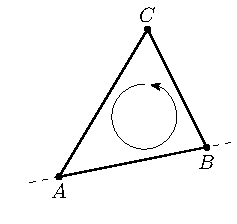
\includegraphics[width=0.7\linewidth]{figures/triangle-counterclockwise.pdf}
      \caption{counterclockwise}
    \end{subfigure}
    % \hfill
    \begin{subfigure}[b]{0.49\linewidth}
      \centering
      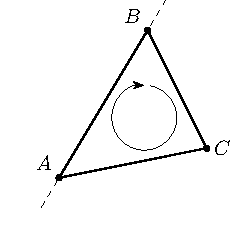
\includegraphics[width=0.7\linewidth]{figures/triangle-clockwise.pdf}
      \caption{clockwise}
    \end{subfigure}
    \caption[Orientations of a Triangle]{%
      \textbf{Orientations of a Triangle}\\
      The images schematically visualize the two distinct orientations of a triangle that correspond to the chosen triangle normal.
      They are given with respect to the outwards-pointing normal of the Euclidean plane and switch when referring to the inwards-pointing normal.
    }
    \label{fig:triangle-orientations}
  \end{figure}

  \begin{definition}[Oriented Triangle]
    An oriented triangle is tuple $\triangle_{[π]} \define (\triangle, [π])$ consisting of a triangle $\triangle$ and an orientation $[π]\in \Theta(\triangle)$.
    The set of directed edges of $\triangle_{[π]}$ is defined as follows.
    % Let $\triangle$ be a triangle and $[π]\in Π(\triangle)/\sim$ be an orientation of $\triangle$.
    % The oriented
    % \[
    %   \triangle_{[π]} \define (\triangle, [π])
    % \]
    \[
      \mathscr{E}(\triangle_{[π]}) \define \set{\overrightarrow{π_1π_2},\overrightarrow{π_2π_3}, \overrightarrow{π_3π_1}}{}
    \]
  \end{definition}
  An oriented triangle is a triangle that has been equipped with an orientation.
  In this sense, it is an oriented topological 2-manifold with an oriented boundary.
  Its oriented boundary can be characterized by the union of its directed edges.
  The structure of an oriented triangle can be modeled by a directed graph connecting its vertices by its directed edges.



  \begin{definition}[Polyhedral Surface and Surface Mesh]
    Let $n\in\setNatural$ with $n\geq 2$ and $\mathscr{T}\neq\emptyset$ be a finite set of triangles embedded in $\setReal^n$.
    Let $S=\bigcup\mathscr{T}$ be a two-dimensional topological manifold (with boundary), such that for all $\triangle_1,\triangle_2\in\mathscr{T}$ with $\triangle_1\neq\triangle_2$ the following holds.
    \[
      \triangle_1\cap\triangle_2 \in \set{\emptyset}{} \cup [\mathscr{V}(\triangle_1)\cap\mathscr{V}(\triangle_2)] \cup [\mathscr{E}(\triangle_1)\cap\mathscr{E}(\triangle_2)]
    \]
    In this case, $S$ is called a (topological) polyhedral surface (embedded in $\setReal^n$).
    With $\mathscr{V}(S)$ we denote its vertices, with $\mathscr{E}(S)$ its edges, and with $\mathscr{F}(S)$ its faces.
    \[
      \mathscr{V}(S) \define \bigcup_{\triangle\in\mathscr{T}} \mathscr{V}(\triangle)
      \separate
      \mathscr{E}(S) \define \bigcup_{\triangle\in\mathscr{T}} \mathscr{E}(\triangle)
      \separate
      \mathscr{F}(S) \define \mathscr{T}
    \]
    % (topological) surface mesh.
    For a clear distinction to the polyhedral surface itself, the following set is called the (topological) surface mesh.
    \[
      \mathscr{M}(S) \define \textstyle\bigcup \mathscr{E}(S)
    \]
    % \[
    %   \partial\mathscr{E}(S) \define \set{e\in\mathscr{E}(S)}{\exists!\triangle\in\mathscr{F}(S)\colon e\subset\triangle}
    %   \separate
    %   \mathscr{E}^\circ(S) \define \mathscr{E}(S) \setminus \partial\mathscr{E}(S)
    % \]
    % \[
    %   \partial S \define \textstyle\bigcup \partial\mathscr{E}(S)
    %   \separate
    %   \partial\mathscr{V}(S) \define \mathscr{V}(S) \cap \partial S
    %   \separate
    %   \mathscr{V}^\circ(S) \define \mathscr{V}(S) \setminus \partial\mathscr{V}(S)
    % \]
  \end{definition}
  The definition makes sure that each pair of triangles may only share a common vertex or edge and does not overlap in any other way.
  Additionally, requiring that the polyhedral surface is a topological 2-manifold, lets neighborhoods of any point be parameterized by two-dimensional charts.
  So, an edge, for example, may only belong either to one or two triangles at the same time.
  I also included a rather uncommon distinction of surface meshes and polyhedral surfaces.
  Whereas the polyhedral surface describes the topological manifold, the surface mesh is the topological model of the underlying graph connecting the vertices of the surface by edges.
  This is done mainly for consistency and convenience when classifying curves.

  For further convenience, my definition of polyhedral surfaces is more restricted than the one of \textcite{polthier2006} as it does not allow for an infinite amount of triangles or arbitrary flat intrinsic metrics.
  Concerning the applications of curve smoothing algorithms, this is not a serious constraint because real-world surfaces in the mesh processing context will always have a finite extent and only allow for finitely many faces.

  For the construction of orientation, I will build on the tools given above for oriented triangles.
  The idea is to consistently choose orientations for every triangle such that the boundary of two adjacent triangles keeps to be an oriented topological 1-manifold --- the orientations are called compatible.
  As it can be seen in figure~\ref{fig:compatible-triangle-orientations}, the orientations of adjacent triangles are only compatible if they do \textit{not} share any directed edge.

  \begin{figure}[t]
    \centering
    \begin{subfigure}[b]{0.49\linewidth}
      \centering
      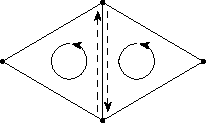
\includegraphics[width=0.8\linewidth]{figures/compatible-triangle-orientations.pdf}
      \caption{compatible}
    \end{subfigure}
    \hfill
    \begin{subfigure}[b]{0.49\linewidth}
      \centering
      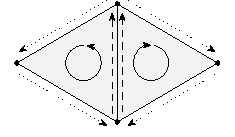
\includegraphics[width=0.8\linewidth]{figures/incompatible-triangle-orientations.pdf}
      \caption{incompatible}
    \end{subfigure}
    \caption[Compatible and Incompatible Triangle Orientations]{%
      \textbf{Compatible and Incompatible Triangle Orientations}\\
      The images schematically visualize compatible and incompatible orientations of two adjacent triangles that share a common undirected edge.
      For compatible orientations, the triangles are not allowed to share a directed edge such that the boundary of their union is again an oriented topological 1-manifold.
    }
    \label{fig:compatible-triangle-orientations}
  \end{figure}

  \begin{definition}[Oriented Polyhedral Surface]
    Let $S$ be a polyhedral surface. Then $S$ is called orientable if there exists a function $\function{ϑ}{\mathscr{F}(S)}{\bigsqcup_{\triangle\in\mathscr{F}(S)} \Theta(\triangle)}$ that selects an orientation for each contained triangle with the following property.
    \[
      \forall \triangle_1,\triangle_2\in\mathscr{F}(S),\triangle_1\neq\triangle_2\colon\quad \mathscr{E}(ϑ(\triangle_1)) \cap \mathscr{E}(ϑ(\triangle_2)) = \emptyset
    \]
    In this case, $ϑ$ is called an orientation of $S$ and $(S,ϑ)$ an oriented polyhedral surface. The set of all orientations for $S$ is denoted with $\Theta(S)$.
  \end{definition}
  \noindent
  % To construct an orientation for a whole polyhedral surface, orientations for all its faces need to be selected first.
  In the case of compatible orientations, two adjacent triangles exhibit the same outer normal when unfolded into the Euclidean plane.
  For connected polyhedral surfaces without boundary, the outer normal of each face then consistently points to the outside or inside of the circumscribed volume depending on the chosen orientation.

  There are artificial cases, such as the polyhedral Möbius strip, of non-orientable polyhedral surfaces.
  Also objects may look like orientable surfaces but may provide artifacts in their surface meshes originating from scanning.
  As polyhedral surfaces are not required to be connected, more than two orientations might exist.

  Especially in this thesis, all algorithms will be constructed for oriented polyhedral surfaces to facilitate their implementation and efficiency.
  Concerning real-world data, this is not an actual restriction.
  Unorientable surface meshes mostly arise from artificial construction or numerical errors that can be handled by other mesh preprocessing techniques.
  For applications that need to process surface meshes, the surfaces mostly are the boundary of finite volumes in three-dimensional Euclidean space.
  These volumes can be viewed as open submanifolds of $\setReal^3$
  Because the Euclidean space itself is oriented, these volumes and, as a consequence, their boundaries need to be oriented, too (see appendix~\ref{sec:analysis_on_manifolds}).

  In analogy to the previous subsection about curves on smooth manifolds, I will also introduce discrete curves on the surface mesh of polyhedral surfaces.
  This will allow for the discretization of geodesics and the geodesics problems.

  \begin{definition}[Surface Mesh Curve]
    Let $S$ be a polyhedral surface, $n\in\setNatural$, and $x\in \mathscr{M}(S)^{n+1}$ be a sequence of control points, such that the following property is fulfilled.
    \[
      % \forall k\in\setNatural,k\leq n\colon x_k\neq x_{k+1} \land \exists \triangle\in\mathscr{F}(S)\colon x_k, x_{k+1}\in\triangle
      \forall k\in\setNatural,k\leq n\colon \exists \triangle\in\mathscr{F}(S)\colon \quad x_k, x_{k+1}\in\triangle
    \]
    The (topological) curve given by connecting adjacent points by a straight line is called the surface mesh curve.
    \[
      \function{γ}{[0,n]}{S}
      \separate
      γ(t) \define \roundBrackets{\floorBrackets{1+t} - t} x_{1 + \floorBrackets{t}} + \roundBrackets{t - \floorBrackets{t}} x_{1 + \ceilBrackets{t}}
    \]
  \end{definition}
  In this definition, control points of a curve are only allowed to lie on edges or vertices of the underlying polyhedral surface.
  To make sure that the connection of two adjacent control points by a straight line is also part of the polyhedral surface itself, they are forced to be part of the same face.
  Mathematically, this property is important for consistency.

  % \begin{corollary}
  %   Discrete surface mesh curves of a polyhedral surface are part of that surface.
  % \end{corollary}
  % \begin{corollary}[Closed Surface Mesh Curves]
  %   γ is closed iff $x_1 = x_{n+1}$
  % \end{corollary}

  Unfortunately, surface mesh curves may still exhibit artifacts, as many adjacent control points might be defined as part of the same triangle.
  These artificial cases do not facilitate the design of curves for mesh processing or other applications and, in general, cannot be handled in an efficient way by algorithms.
  So, I will strive for using surface mesh curves without artifacts.

  \begin{definition}[Regular Surface Mesh Curve]
    Let $S$ be a polyhedral surface and γ be a surface mesh curve characterized by the control point sequence $x\in\mathscr{M}(S)^{n+1}$ with $n\in\setNatural$.
    If γ is open, it is called regular if the following property holds.
    \[
      \forall k\in\setNatural, 1 < k \leq n\colon \quad
      % \mathscr{F}_S(x_{k-1}) \cap \mathscr{F}_S(x_{k+1}) = \emptyset
      \forall \triangle\in\mathscr{F}(S) \colon \quad x_{k-1}\not\in\triangle \ \vee\  x_{k+1}\not\in\triangle
    \]
    In the case that γ is a closed curve (ie. $x_1 = x_{n+1}$), γ is regular if it additionally fulfills the following boundary condition.
    \[
      % \mathscr{F}_S(x_1) \cap \mathscr{F}_S(x_n) = \emptyset
      \forall \triangle\in\mathscr{F}(S) \colon \quad x_{2}\not\in\triangle \ \vee\  x_{n}\not\in\triangle
    \]
  \end{definition}
  By forbidding three adjacent control points to lie on the same triangle, surface mesh curves without artifacts are representable a by a sequence of $n$ triangles, $n-1$ real values, and start/end points.
  In this representation, control points lie on the common edges of two adjacent triangles.

  At first, the concept of discrete surface mesh curves is much more restricted than the standard practice of using piecewise continuously differentiable curves as it was done by \textcite{polthier2006}.
  Still, regular surface mesh curves can represent all geodesics, are robust when it comes to singularities, and more efficient.
  Should there be need for more fine-grained curve smoothing inside single faces, a retriangulation should be triggered.
  Furthermore, in the context of this thesis, polyhedral surfaces are not understood to be approximations of smooth manifolds, it would not be consistent to allow arbitrarily bended curves inside a single face.

  To make it possible to use regular surface mesh curves for the definition of discrete geodesics, \textcite{polthier2006} introduce the concept of discrete geodesic curvature.

  \begin{definition}[Total Vertex Angle]
    Let $S$ be a polyhedral surface.
    For vertices $v\in\mathscr{V}(S)$, the total vertex angle is defined as follows.
    \[
      ϑ_\triangle(A) = \arccos\frac{\scalarProduct{\overrightarrow{AB}}{\overrightarrow{AC}}}{\norm{\overrightarrow{AB}}\norm{\overrightarrow{AC}}}
    \]
    \[
      ϑ_S(v) \define \sum_{\triangle\in\mathscr{F}(S), v\in\triangle} ϑ_\triangle(v)
    \]
  \end{definition}

  Surface mesh curves without artifacts will never contain points that lie on the inside of a boundary edge.
  They may contain boundary vertices.

  \begin{definition}[Curve Angle]
    Let $S$ be a polyhedral surface and $p,x,q\in\mathscr{M}(S)$, $x\in S^\circ$ be adjacent vertices of surface mesh curve without artifacts on $S$.
    Let $\mathscr{V}_S(x)$ the neighboring vertices.
    The neighbor set can be partitioned into three possible empty tuples, such that $p,(x),q$ is surface mesh curvature without artifacts.
    There exists two tuples $(p=x_{λ(0)},x_{λ(1)},\ldots,x_{λ(n)},x_{λ(n+1)} = q)$ and $(p,x_{ρ(1)},\ldots,x_{ρ(m)},q)$ that characterize a surface mesh curve without artifacts.
    \[
      β_λ = \sum_{k=1}^n \sphericalangle(x_{λ(k-1)},x_{λ(k)},x_{λ(k+1)})
      \separate
      β_ρ = \sum_{k=1}^m \sphericalangle(x_{ρ(k-1)},x_{ρ(k)},x_{ρ(k+1)})
    \]
    The (unoriented) curve angle at $x$ is given by the sum
    \[
      β = \min \set{β_λ, β_ρ}{}
    \]
    If there is an orientation $Π$ for $S$ then the (oriented) curve angle is given by the segmentation which points are connected by directed edge paths in their respective triangles such that $x$ is not contained.
  \end{definition}
  For the oriented case, the curve angle can only be defined for curve vertices that do not lie on the boundary of $S$.
  Also the interpretation of the total vertex angle for boundary points is different.
  This makes a generalization of the oriented discrete curvature at boundary points difficult.

  \begin{definition}[Discrete Geodesic Curvature]
    \[
      κ_\mathrm{g}(γ) = π - \frac{2π}{ϑ_S(γ)}β_S(γ)
    \]
  \end{definition}

  \begin{definition}[Discrete Geodesic Curvature for Boundaries]

  \end{definition}

  \begin{definition}[Discrete Geodesic Problems]

  \end{definition}

  \begin{lemma}[Straightest and shortest geodesics are surface mesh curves without artifacts.]

  \end{lemma}

% subsection polyhedral_surfaces (end)

% Differential Geometry on Polyhedral Surfaces
% \autocite{polthier2006}

% Curvature Estimation on Surfaces
% \autocite{rusinkiewicz2004}

% Generation of Surface Normals
% \autocite{max1999,meyer2001,jin2005}

% section preliminaries (end)
\end{document}
